\chapter{Results}

% Explain Like I'm 5
% Mention CityCraft on first page of introduction and in abstract as well.
This chapter presents CityCraft, the standalone city generation software that was implemented as a result of this research.
CityCraft is a graphical desktop application that lets users interactively generate 3D cities, which can be exported as glTF files and used in third-party modeling software such as Blender.
The application combines computer graphics theory and several PCG techniques to achieve its results.
An example of CityCraft in use is shown in Figure \ref{fig:screenshot}, and a CityCraft generated model is shown rendered in Blender in Figure \ref{fig:blender}.

\begin{figure}[H]
  \centering
  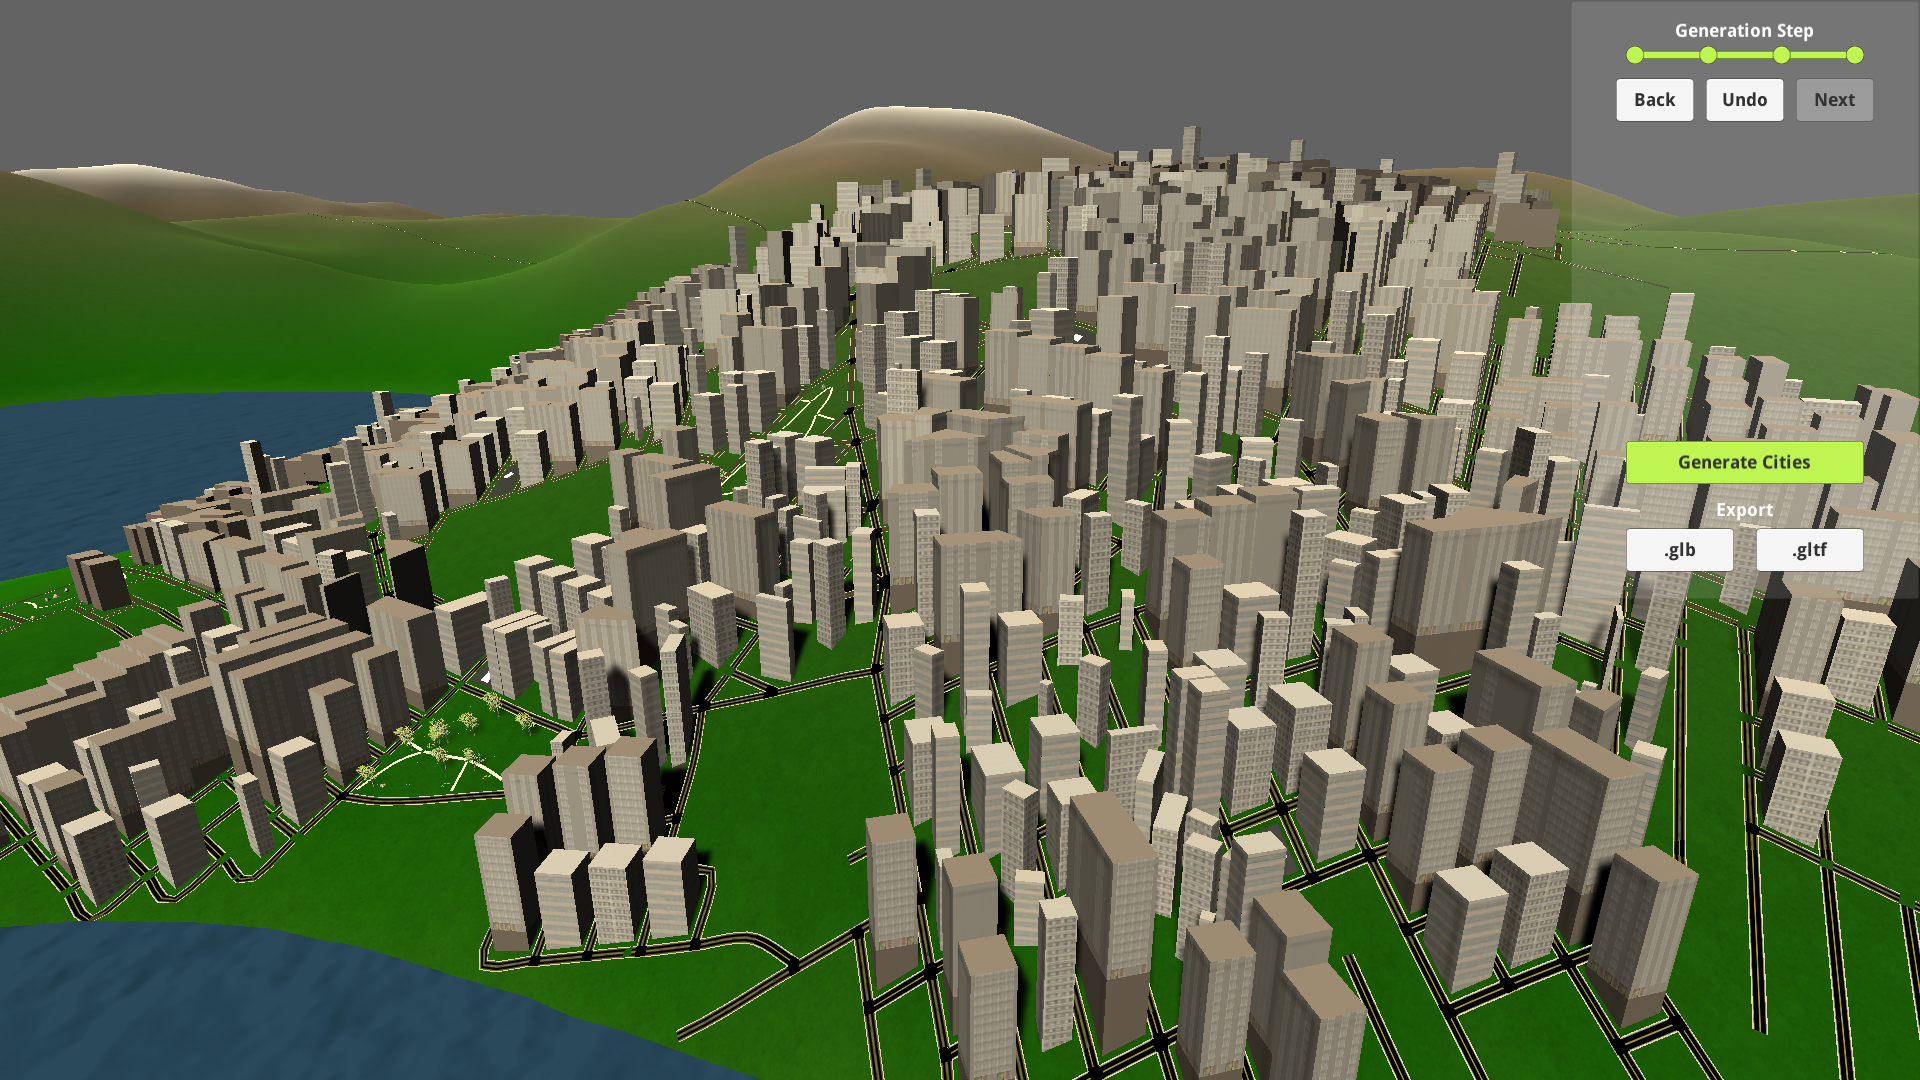
\includegraphics[width=\textwidth]{figure/results/screenshot.png}

  \caption{A screenshot taken from CityCraft as a user generates a city. In the top-right resides a menu panel which the user operates to perform the generation. The view of the world is control through a camera which is rotated with the mouse and moved with the keyboard.}
  \label{fig:screenshot}
\end{figure}

\begin{figure}[H]
  \centering
  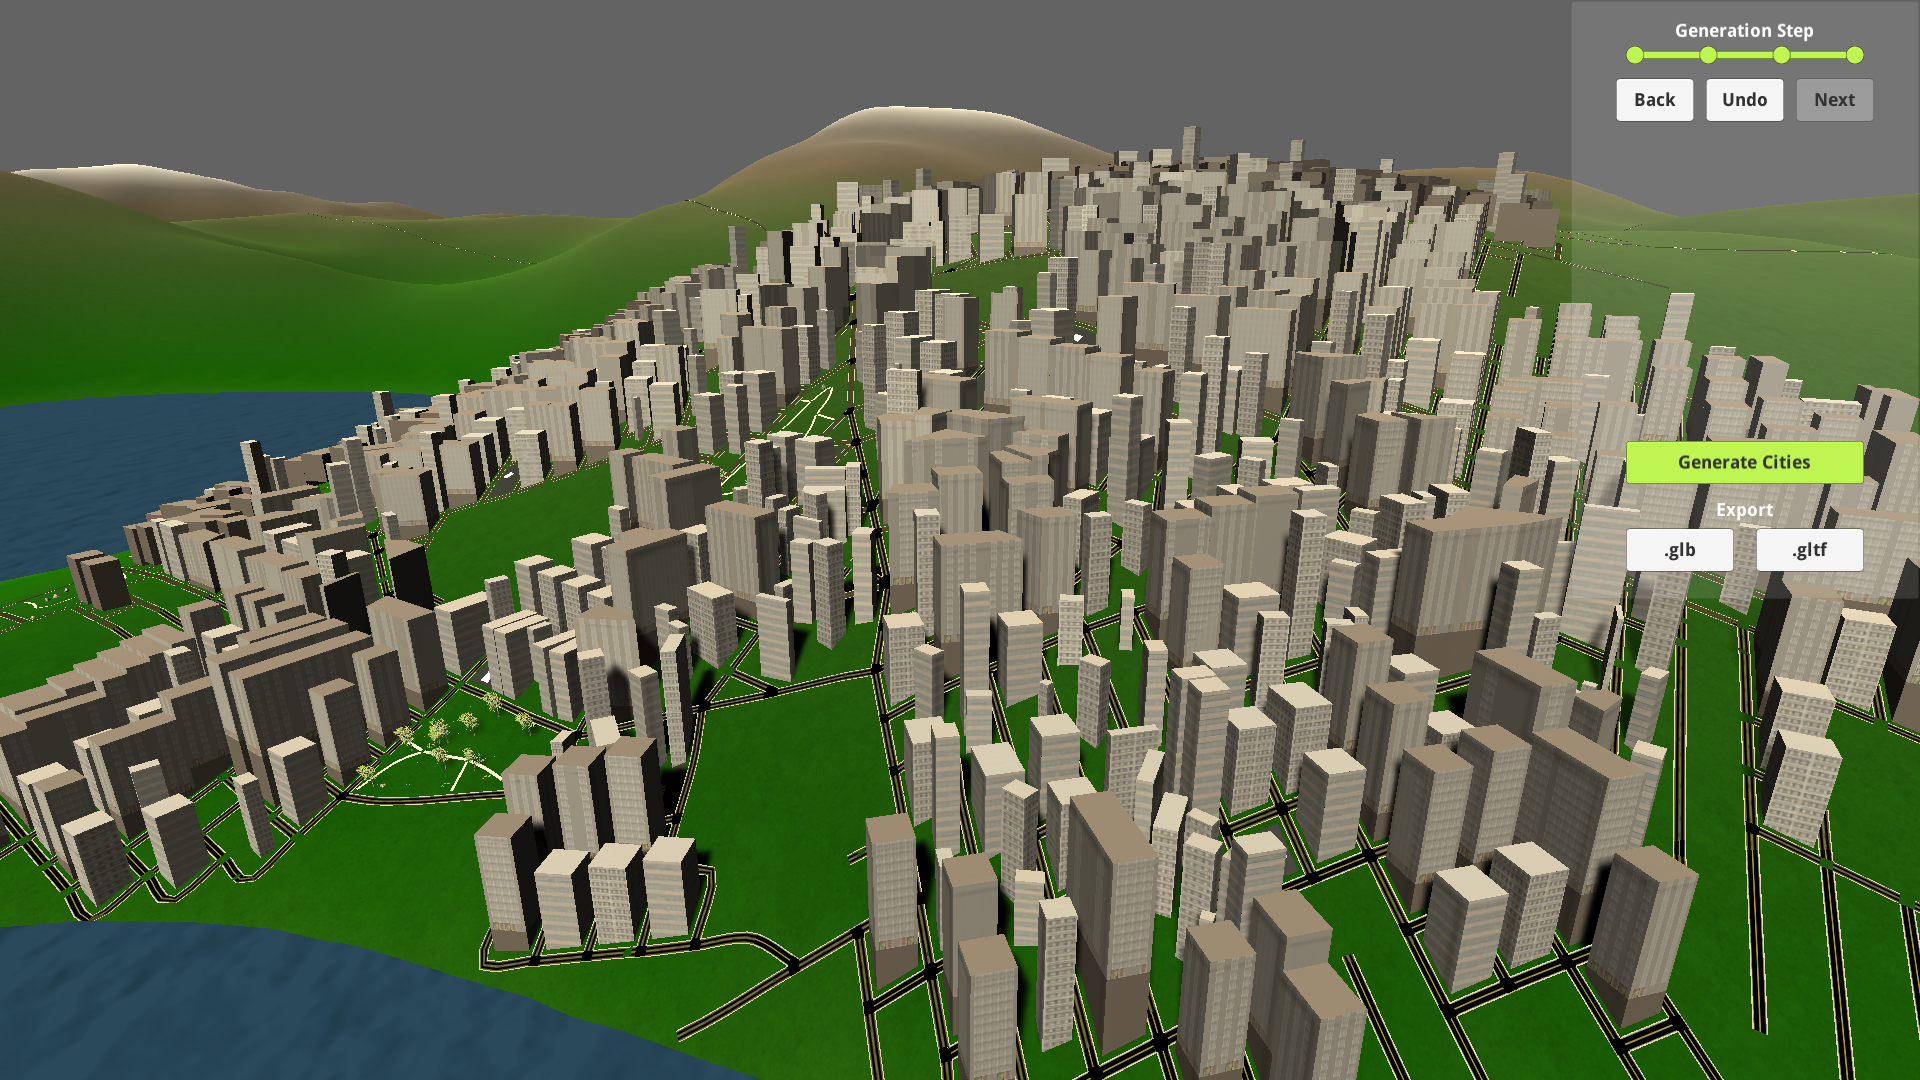
\includegraphics[width=\textwidth]{figure/results/screenshot.png}

  \caption{A city model exported from CityCraft and rendered inside Blender.}
  \label{fig:blender}
\end{figure}

CityCraft's GUI follows the \textit{Wizard} design pattern \cite{yer_a_wizard} to guide its users through the generation process, which is split into four steps (see Figure \ref{fig:guisteps}).
The four generation steps are terrain, roads, streets, and cities.
The last of which performs the generation of buildings, parks, and parking lots. 

\begin{figure}[H]
  \centering
  \begin{subfigure}[b]{0.24\textwidth}
    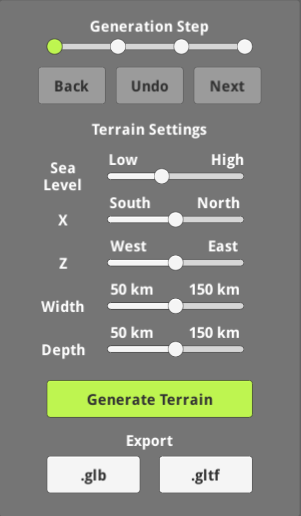
\includegraphics[width=\textwidth]{figure/results/gui1.png}
  \end{subfigure}
  \begin{subfigure}[b]{0.24\textwidth}
    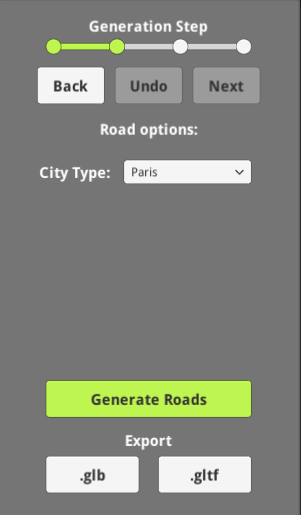
\includegraphics[width=\textwidth]{figure/results/gui2.png}
  \end{subfigure}
  \begin{subfigure}[b]{0.24\textwidth}
    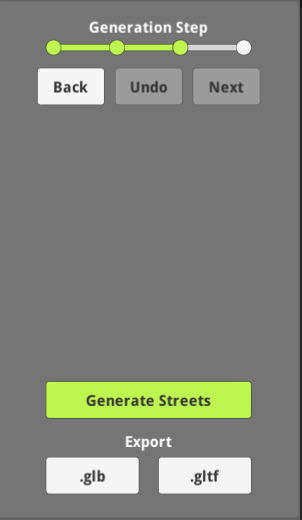
\includegraphics[width=\textwidth]{figure/results/gui3.png}
  \end{subfigure}
  \begin{subfigure}[b]{0.24\textwidth}
    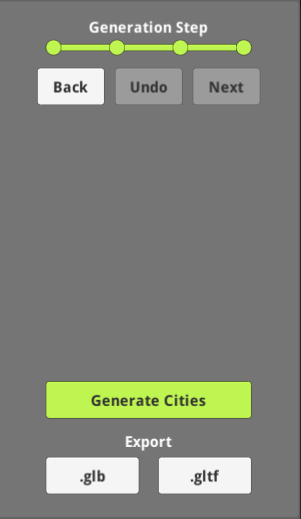
\includegraphics[width=\textwidth]{figure/results/gui4.png}
  \end{subfigure}

  \caption{CityCraft's four steps of generation. Each step has a separate settings panel and each generation can be performed multiple times.}
  \label{fig:guisteps}
\end{figure}

The four generation steps of the GUI are implemented as eight PCG-based generators, all of which are orchestrated by a single module called the \textit{WorldGenerator}.
The following subchapters will go into detail about the results that each of these generators produces and how their results contribute to the final city models.

\section{Terrain Generation}

When users start CityCraft, they are first presented with an endless ocean and a menu panel, as shown in Figure \ref{fig:no_terr}.
This is the start of the generation process, and the ocean represents the blank canvas on which the rest of the world will be built.

\begin{figure}[H]
  \centering

  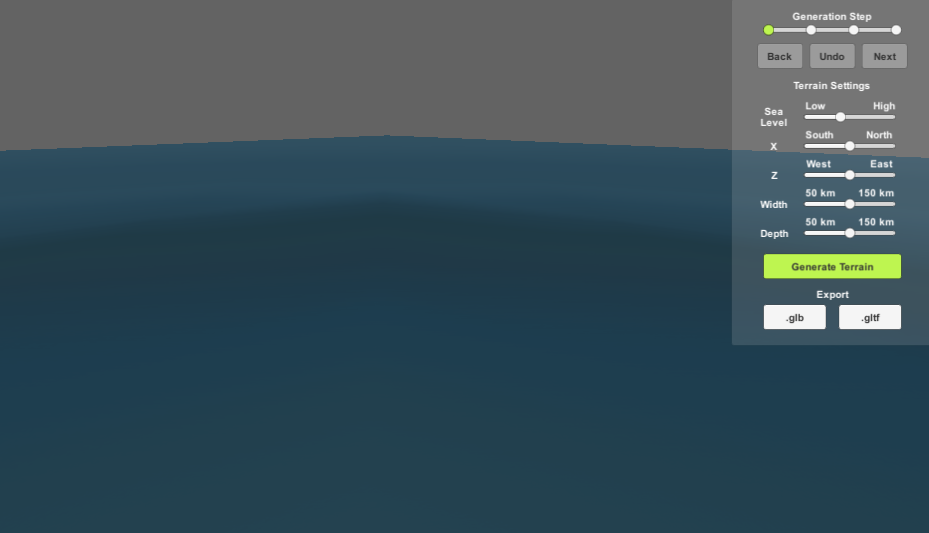
\includegraphics[width=0.7\textwidth]{figure/terrain_not_generated.png}
  \caption{The application state before the \textit{Generate Terrain} button has been pressed. The ocean is visible from the very beginning.}

  \label{fig:no_terr}
\end{figure}

The very first step of the generation processs is to generate the terrain, whose settings are adjusted in the top-right menu panel.
The terrain settings that the user can adjust are:
\begin{easylist}
  @ Sea level: modifies the water level.
  @ X/Z offset: offsets the sampling location along respective axis of the noise function, effectively changing the height values of the terrain.
  @ Width/Depth: adjusts the size of the entire terrain.
\end{easylist}

The terrain is generated by creating a surface mesh whose vertices are given height values sampled from a 4-layered Simplex noise function.
The terrain utilizes a single texture, which is repeated several times with randomized UV coordinates.
The terrain is also colored based on height values, forming snowy mountain tops and green valleys.
An example of a generated terrain is shown in Figure \ref{fig:terr}.

\begin{figure}[H]
  \centering

  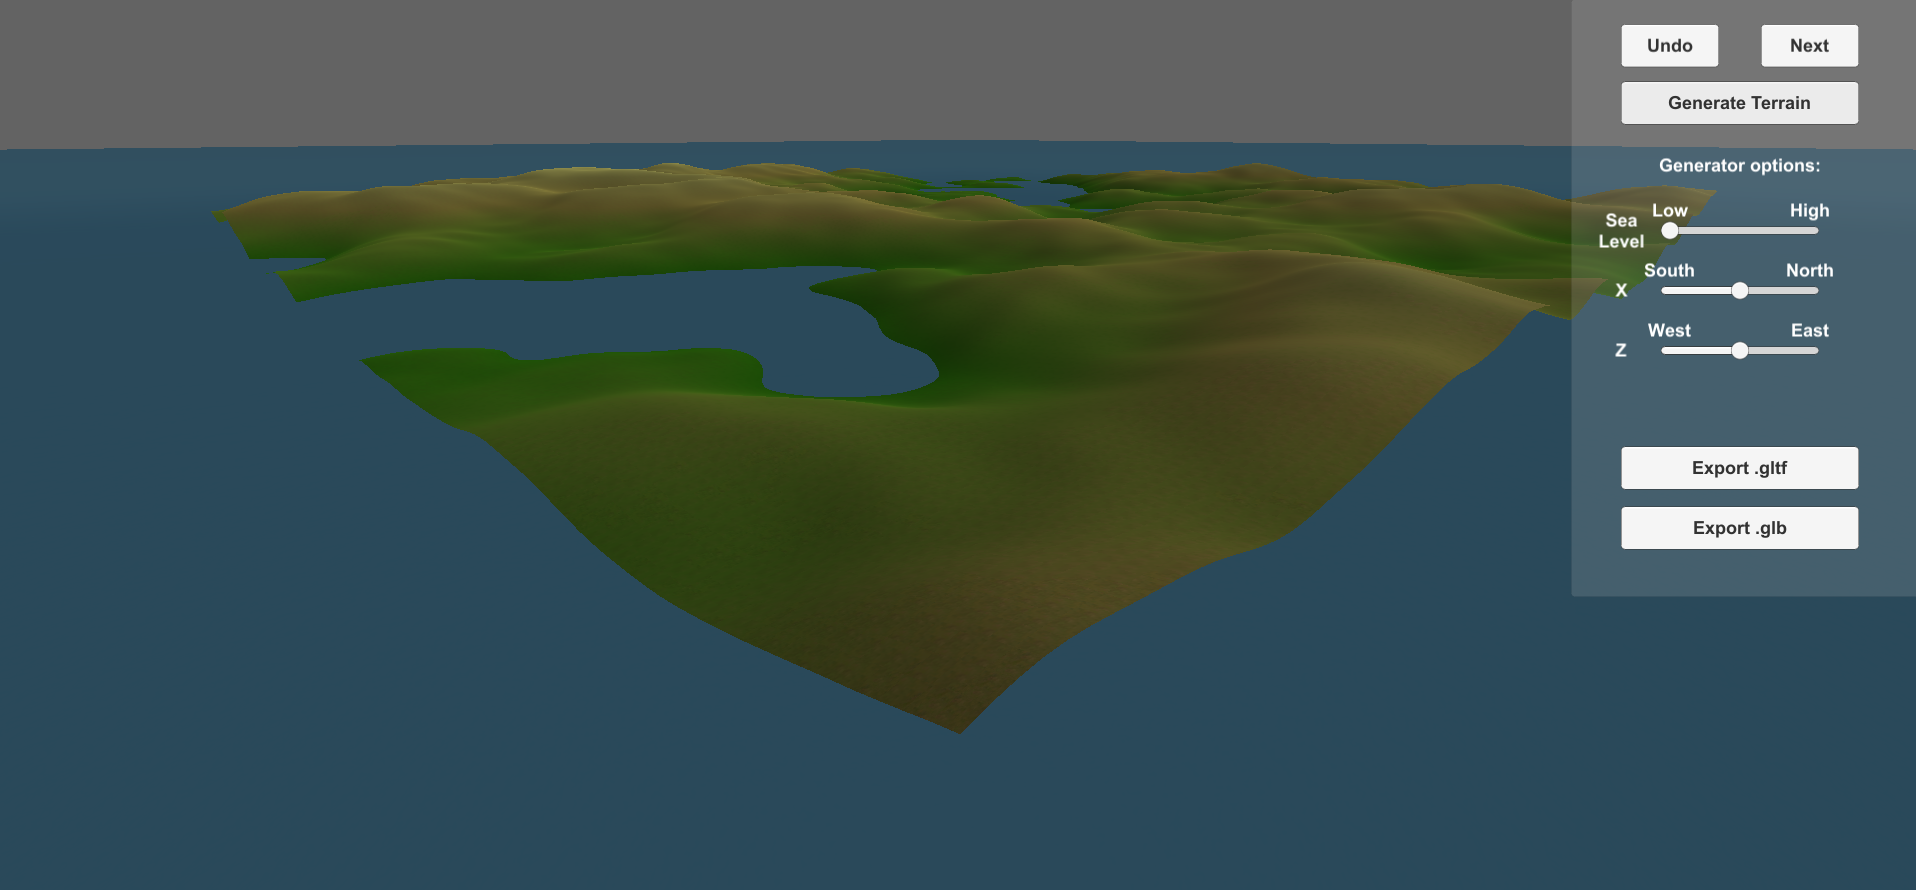
\includegraphics[width=0.7\textwidth]{figure/terrain_generated.png}
  \caption{The application state after \textit{Generate Terrain} has been pressed. The user may change settings and regenerate the terrain as many times as they like.}

  \label{fig:terr}
\end{figure}

The ocean was just implemented as a large textured plane that clips through the terrain, forming lakes at its intersections.


\section{Population Generation}
\section{Road Generation}

After the city markers are specified and the population density map has been created, it is time to generate the road network.
Using the markers, the road generator creates workers called Agents in the area specified by the markers and assigns them strategies depending on the corresponding city type.
The purpose of the strategies is solely to give Agents instructions for movement and termination.
Strategies take a few different variables into account when it decides these actions, for example the amount of steps an Agent has taken so far, the population density, and if the Agent has landed on an existing road.
The application has Agent strategies for Paris and Manhattan cities, and an example of these are shown in Figure~\ref{fig:results_city_paris} and Figure~\ref{fig:results_city_manhattan}.

How the roads are created and connected is entirely up to the road network.
It handles placing down road nodes and connecting them together, making sure that intersections are created where necessary.
The Agents simply instruct the road network where it wants to place down roads, and the network handles the rest while also providing the Agent with information of how the road network was modified.
Then, the strategies can use that information and react accordingly, for example to terminate the Agent.

From Figure~\ref{fig:results_real_city_manhattan} we can clearly observe the distinct grid-like structure of the road network, which in turn was the goal for our Manhattan generation strategy.
The overall shape of the city does not necessarily mimic the shape of Manhattan in the real world because Manhattan is surrounded by water, something that we are not required to have in our application.
If the city marker is placed on an isolated island, it would be much closer to the aspects of Manhattan in the real world.

\begin{figure}[H]
  \centering
  % Use two minipages to add padding for the figure and its caption
  \begin{minipage}[b]{.455\textwidth}
    \centering
    \begin{minipage}[b]{.9\textwidth}
      \centering
      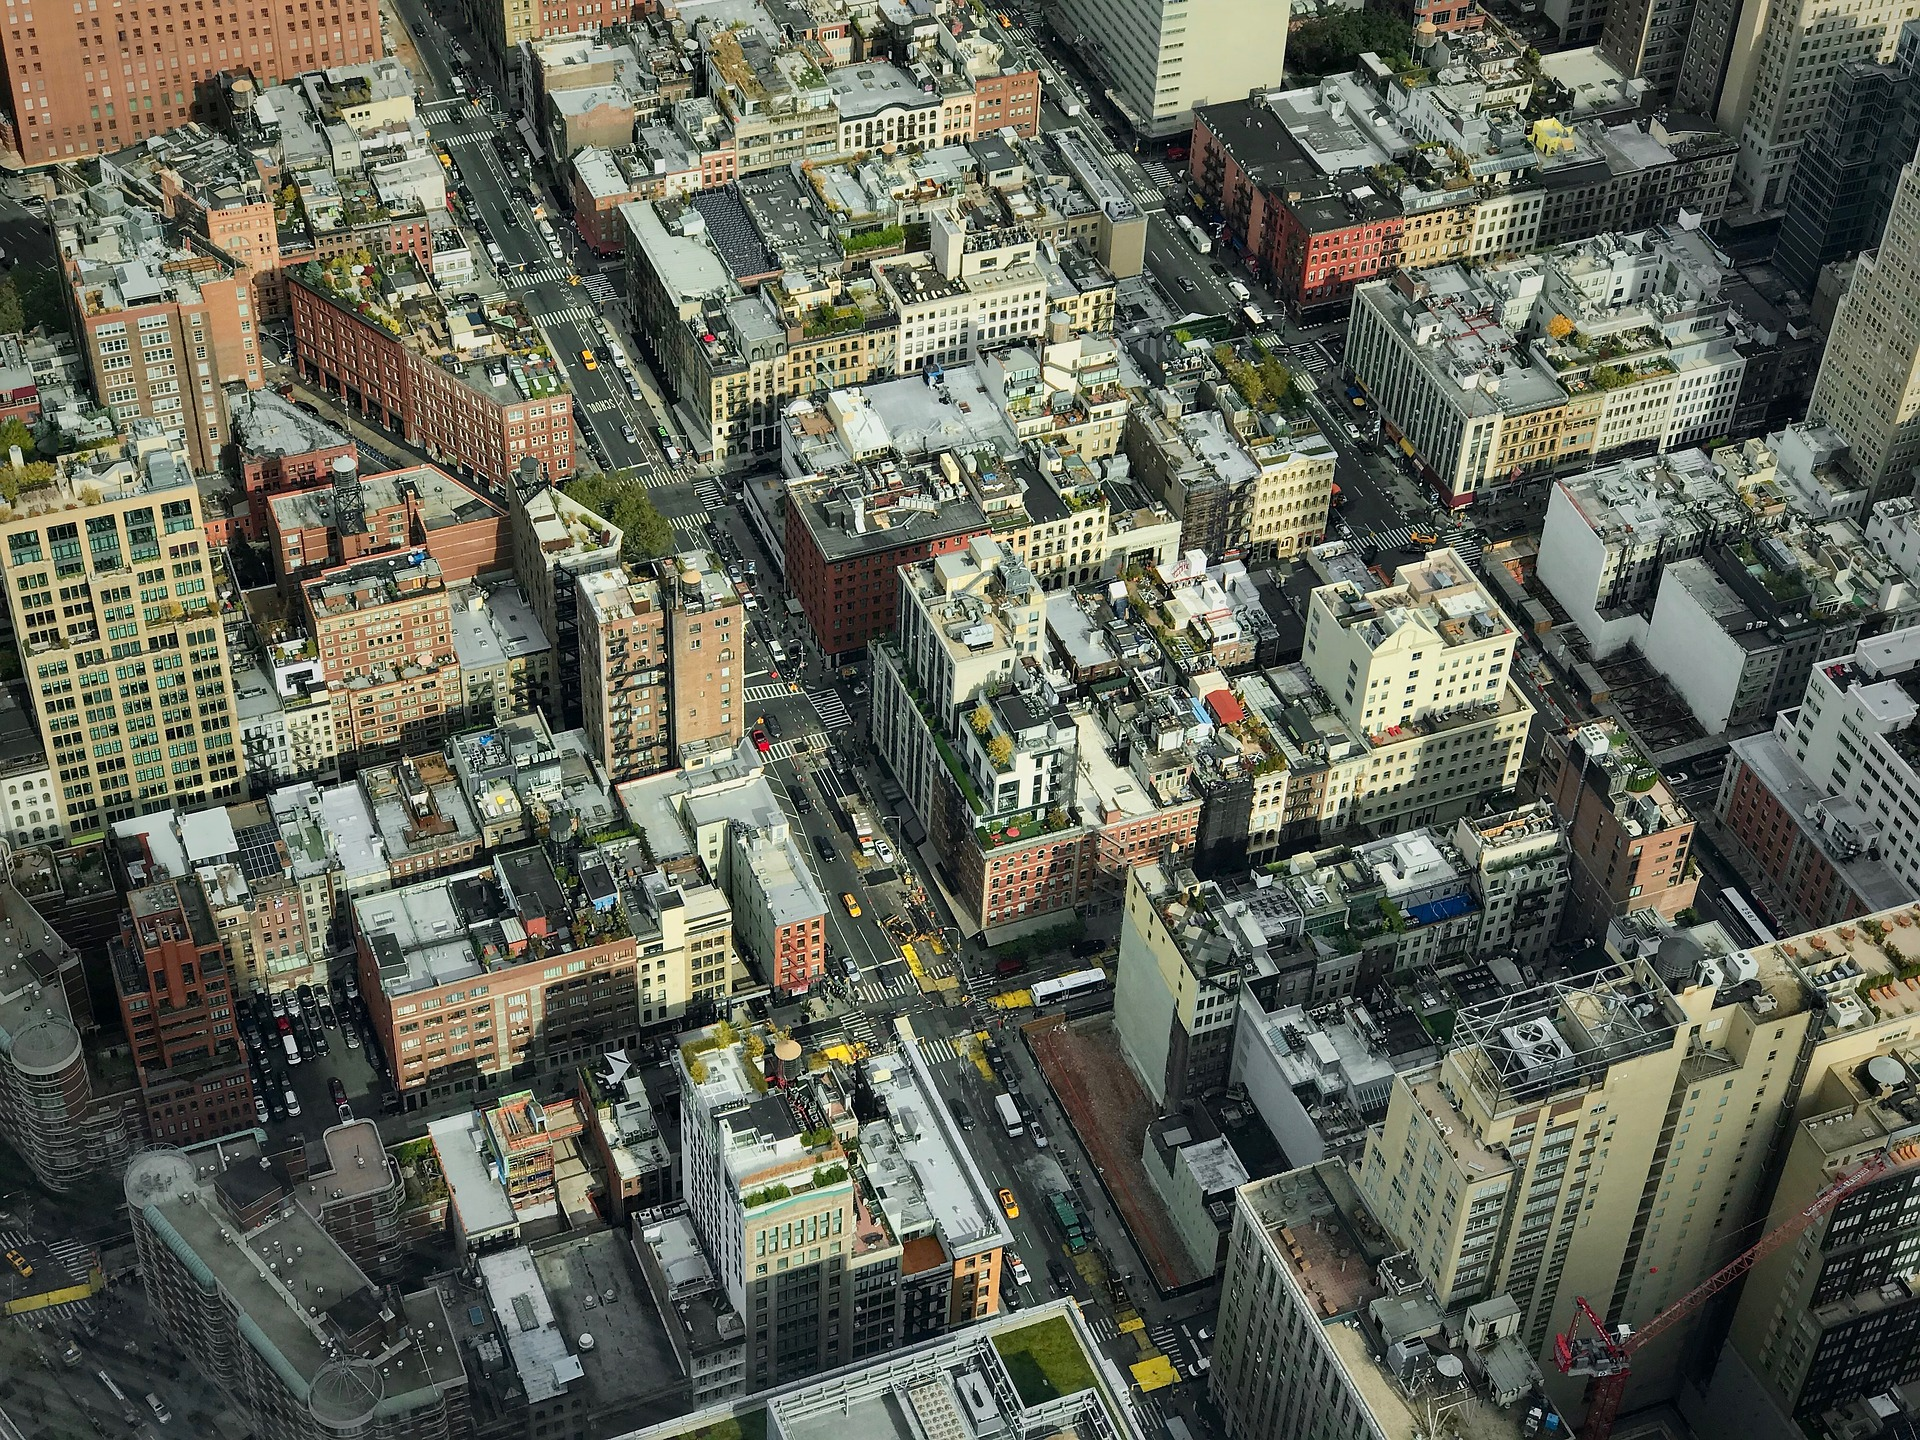
\includegraphics[width=\textwidth]{figure/results/manhattan.jpg}
      \caption{Picture of Manhattan grid-like road system~\cite{manhattan_city_img}.}
      \label{fig:results_real_city_manhattan}
    \end{minipage}
  \end{minipage}
  \begin{minipage}[b]{.445\textwidth}
    \begin{minipage}[b]{.9\textwidth}
      \centering
      \centering
      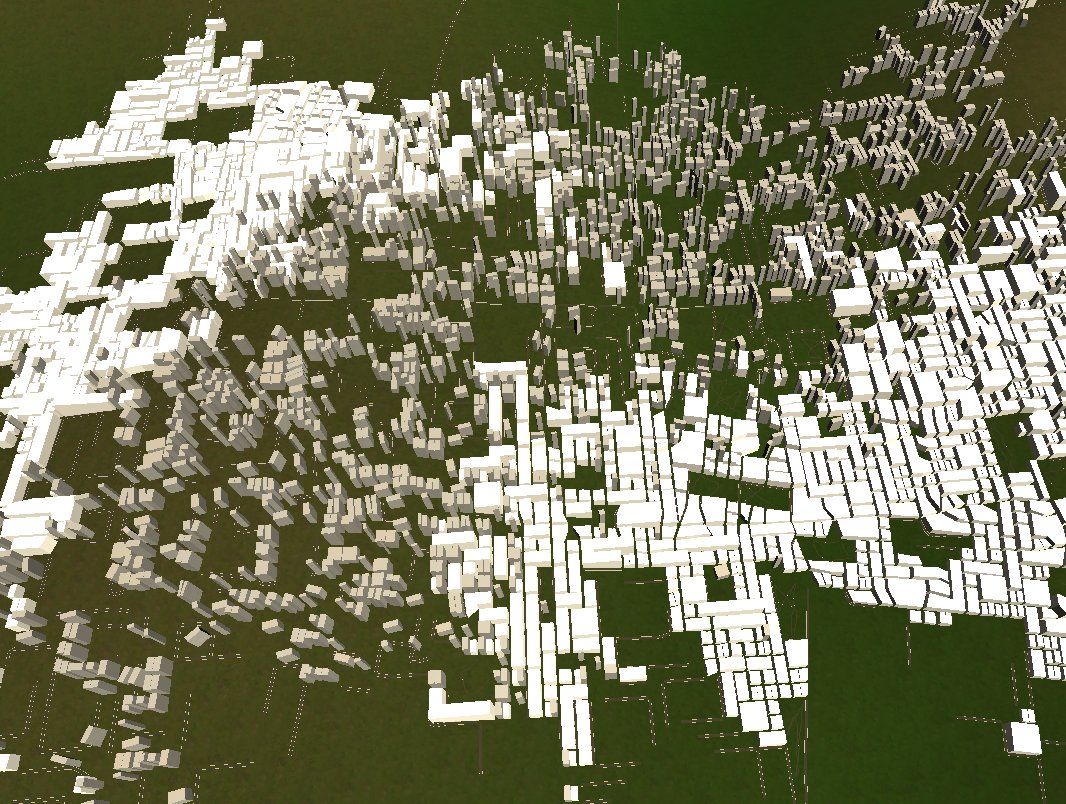
\includegraphics[width=\textwidth]{figure/results/city_manhattan.png}
      \caption{Example of a fully generated Manhattan-style city.}
      \label{fig:results_city_manhattan}
    \end{minipage}
  \end{minipage}
\end{figure}

Meanwhile, Paris has a very different overall aesthetic than Manhattan.
Around the Arc de Triomphe in Figure~\ref{fig:results_real_city_paris}, there are distinct rings and roads extending from the center, which is something we aimed to mimic in this project.
In the generated city in Figure~\ref{fig:results_city_paris}, the structure does have distinct rings and roads similar to the pattern in Paris. 

\begin{figure}[H]
  \centering
  % Use two minipages to add padding for the figure and its caption
  \begin{minipage}[b]{.41\textwidth}
    \centering
    \begin{minipage}[b]{.9\textwidth}
      \centering
      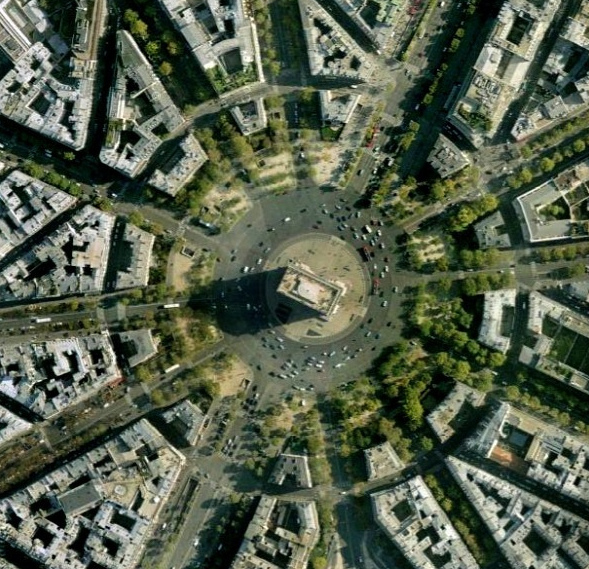
\includegraphics[width=\textwidth]{figure/results/paris_arc_de_triomphe.jpg}
      \caption{Picture of Paris ring-like road system~\cite{paris_city_img}.}
      \label{fig:results_real_city_paris}
    \end{minipage}
  \end{minipage}
  \begin{minipage}[b]{.49\textwidth}
    \begin{minipage}[b]{.9\textwidth}
      \centering
      \centering
      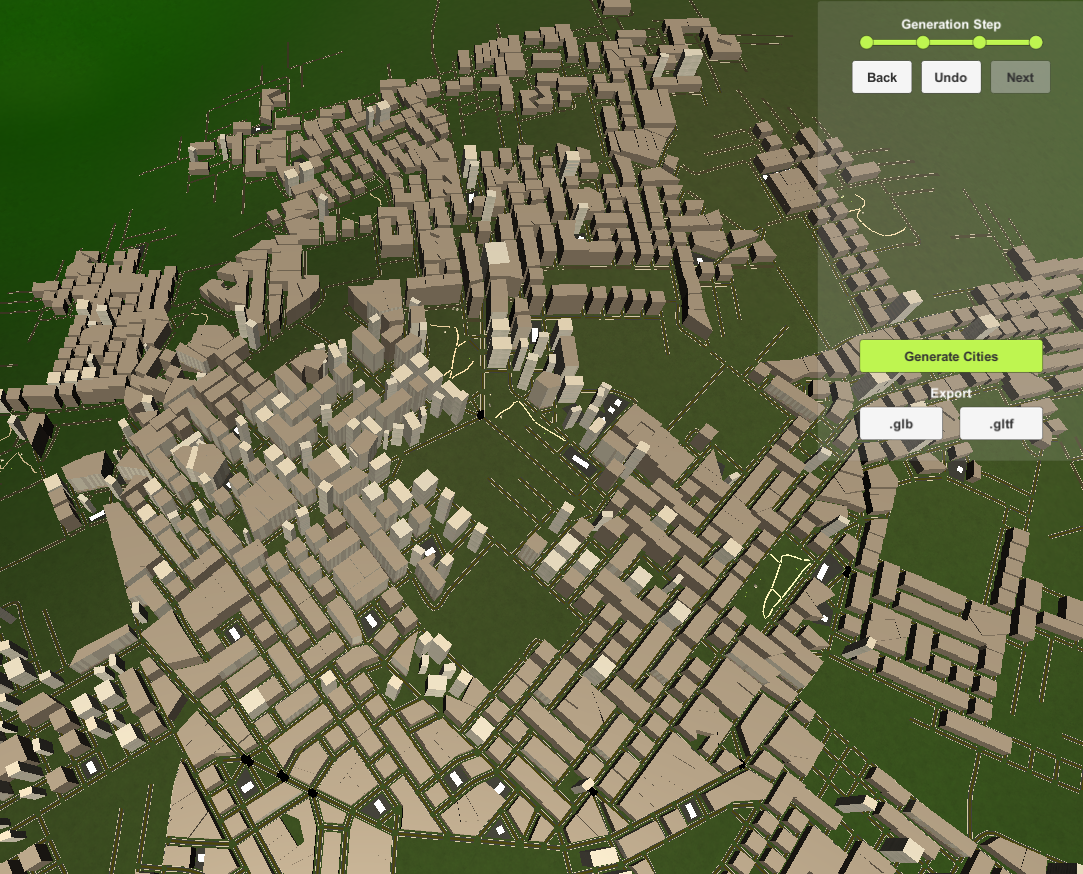
\includegraphics[width=\textwidth]{figure/results/city_paris.png}
      \caption{Example of a fully generated Paris-style city.}
      \label{fig:results_city_paris}
    \end{minipage}
  \end{minipage}
\end{figure}

Both city types have streets branching out from their main roads, which in turn also branch out from themselves to form a grid-like street neighborhood.
These streets are created using a street strategy which is shared between the strategies used for the two different city types, however it is possible to implement more complex street strategies for other types of cities.

The base of the road generator and its strategies allows any kind of street pattern to be produced, given a suitable strategy is implemented.
In order to limit ourselves in this project, the street strategy was implemented to produce grid-like streets for all city types.
However, the configuration of the general street strategy can be configured per city type, which gives a small level of tweaking so the streets could match the city type better.

The generated cities are connected by the road network through what is called highways.
Highways are created by the Agents through highway strategies when they have travelled far away from the designated city markers.
The purpose of the highway strategy is simply to create longer roads with little change in direction.
It also aims to follow the population map density to some degree, especially navigating towards higher populated areas.
This results in highways which typically connect cities together.

\section{City Block Generation}

Once roads and streets have been generated, the city block generation starts.
This generation step produces a list of polygons that mark which areas of the terrain are suitable for buildings, parks, and parking lots to be built on.
City blocks may vary significantly in size but a limit is set on how large they can become (see Figure \ref{fig:results_blockgen1}).

% TODO: Replace this figure, it has some inset problems.
\begin{figure}[h!]
  \centering

  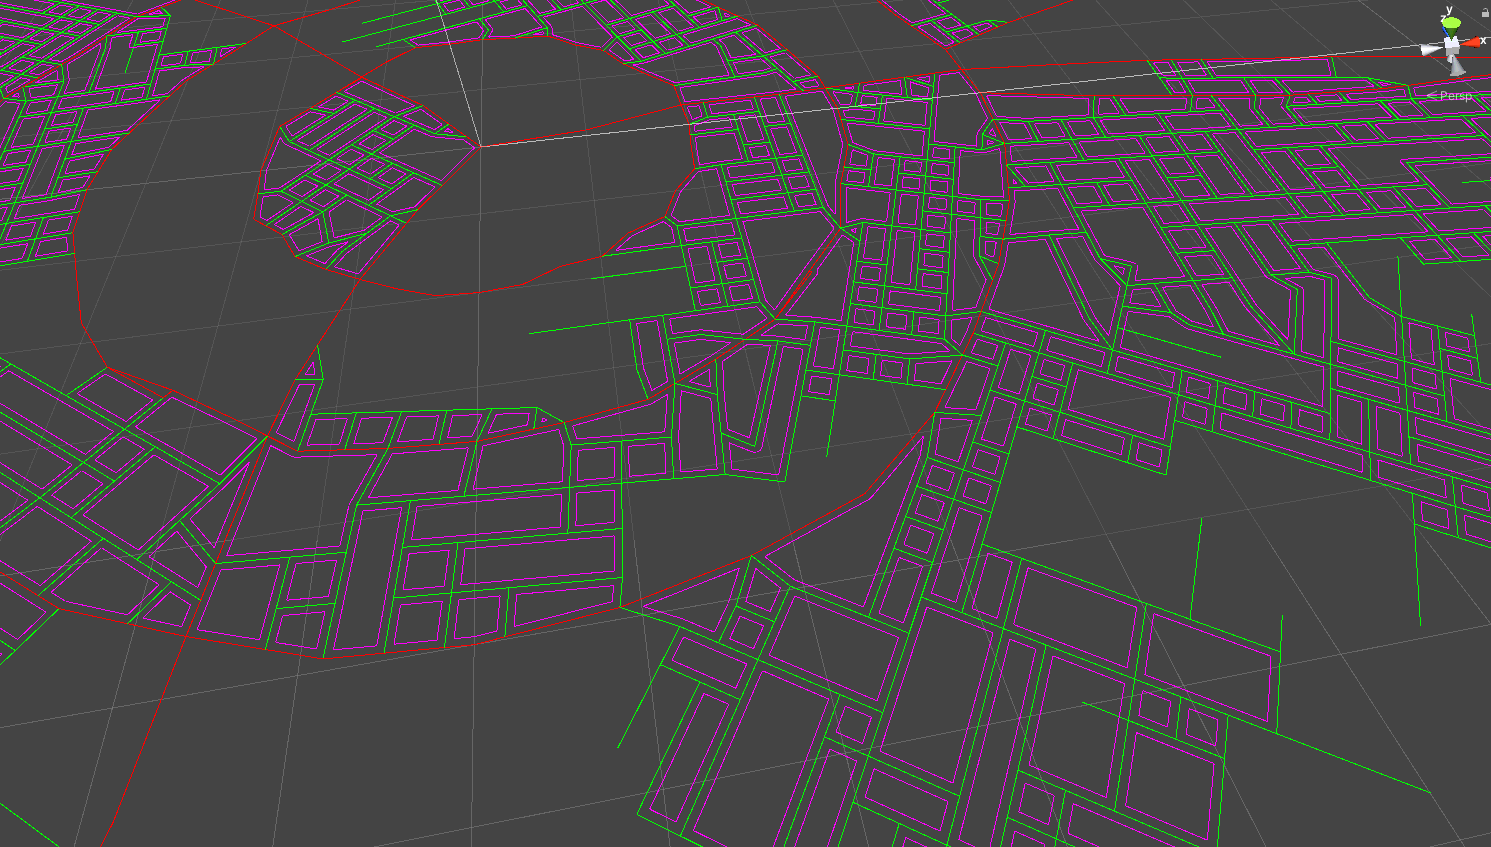
\includegraphics[width=0.8\textwidth]{figure/results_blockgen1.png}
  \caption{Generation of city blocks on a flat road network. Red and green lines represent roads and streets respectively, while pink lines are city blocks. Notice how the largest areas are not treated as blocks.}

  \label{fig:results_blockgen1}
\end{figure}

Each city block is also guaranteed to be connected to the road network, such that it is surrounded by roads and/or streets.
Consequently, each block is slightly inset in order to make room for the road meshes.
This necessity becomes more apparent when all meshes are rendered (see Figure \ref{fig:results_blockgen2}).

\begin{figure}[h!]
  \centering

  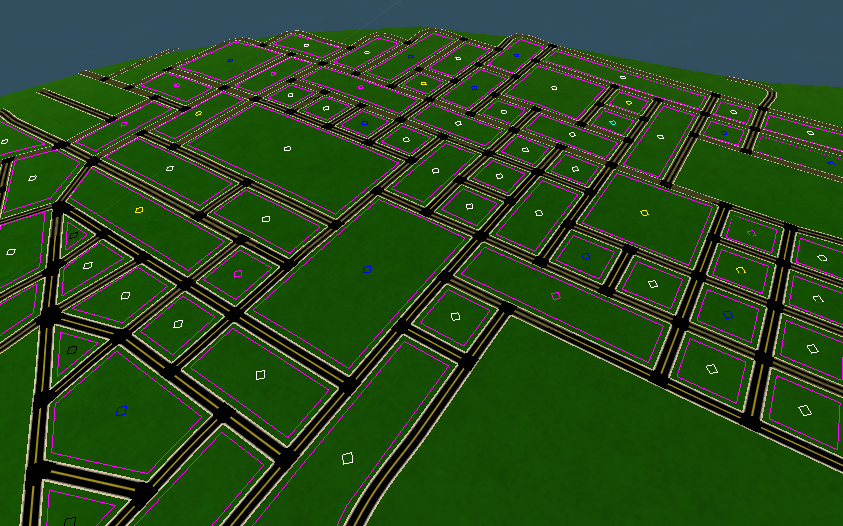
\includegraphics[width=0.9\textwidth]{figure/results_blockgen2.png}
  \caption{Blocks generated on a 3D terrain. Notice how each block is connected to the road network. Green and pink lines are only shown during development.}

  \label{fig:results_blockgen2}
\end{figure}

Each polygon is assigned a label that helps the subsequent Plot Generation step determine what to generate inside each city block.
In Figure \ref{fig:results_blockgen2} these labels are visualized as green triangles, meaning they have not been processed yet.
The green triangles are also used to mark blocks that became too small after being inset, effectively excluding them from further processing.
An example of this behavior is shown in Figure \ref{fig:results_blockgen3}.

\begin{figure}[h!]
  \centering
  \begin{subfigure}[b]{0.47\textwidth}
    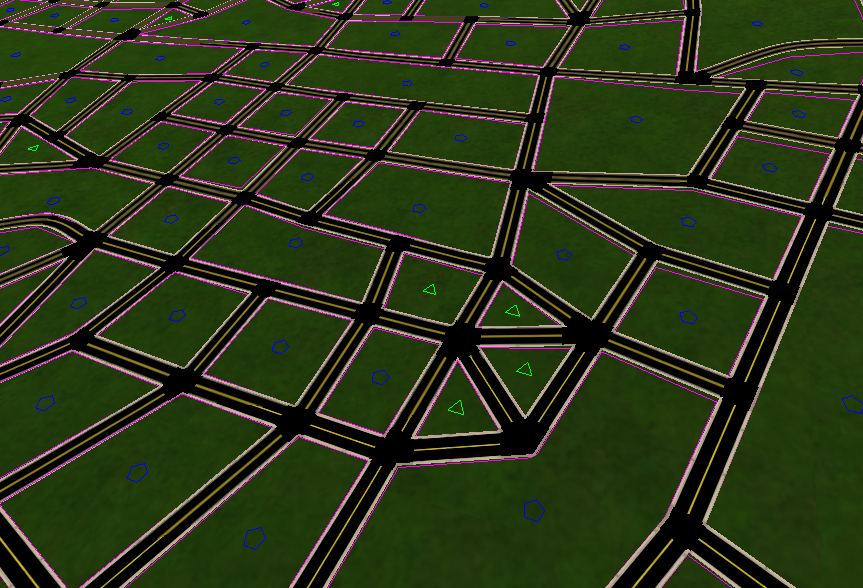
\includegraphics[width=\textwidth]{figure/results_blockgen3.png}
  \end{subfigure}
  \quad
  \begin{subfigure}[b]{0.45\textwidth}
    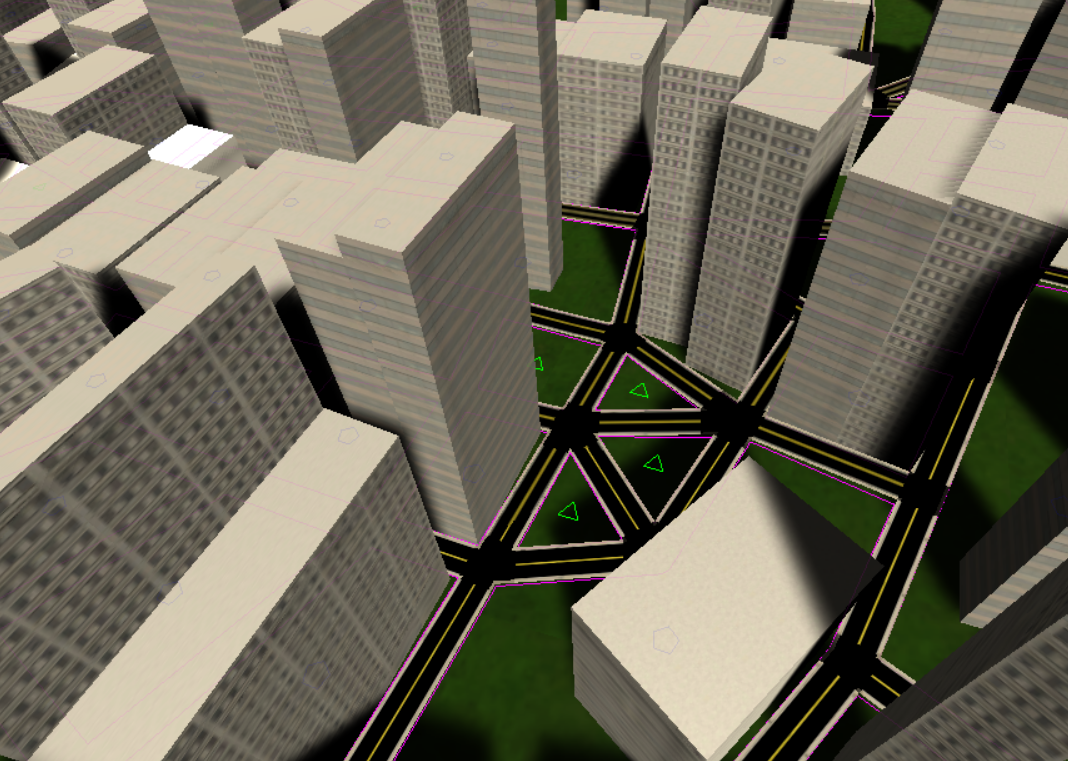
\includegraphics[width=\textwidth]{figure/results_blockgen4.png}
  \end{subfigure}

  \caption{City blocks with different labels (green/blue) shown without (left) and with (right) buildings rendered. Blocks with green labels are too small, and blocks with blue labels are part of the city center.}
  \label{fig:results_blockgen3}
\end{figure}

The generated blocks are then passed on to the plot generation.
\section{Plot Generation}
Each block that is sent into the PlotGenerator is treated differently depending on what the block label is. 
If the block label is either \textit{Parks} or \textit{Parking}, then the PlotGenerator does not split the block. 
The entire block is turned into a plot and is sent to ParkGenerator or ParkingGenerator respecitvely.
The rest of the block labels are split into n parts, where n depends on the area of the block and some randomness. 

In Figure \ref{fig:plot} and \ref{fig:plot2} are examples of the output for the PlotGenerator.

\begin{figure}[H]
  \centering

  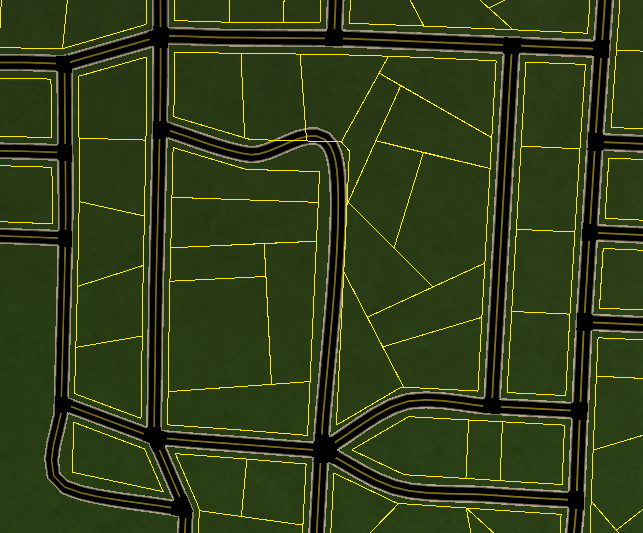
\includegraphics[width=0.8\textwidth]{figure/plot2.png}
  \caption{Close-up of the plot splitting algorithm.}

  \label{fig:plot2}
\end{figure}

\begin{figure}[H]
  \centering

  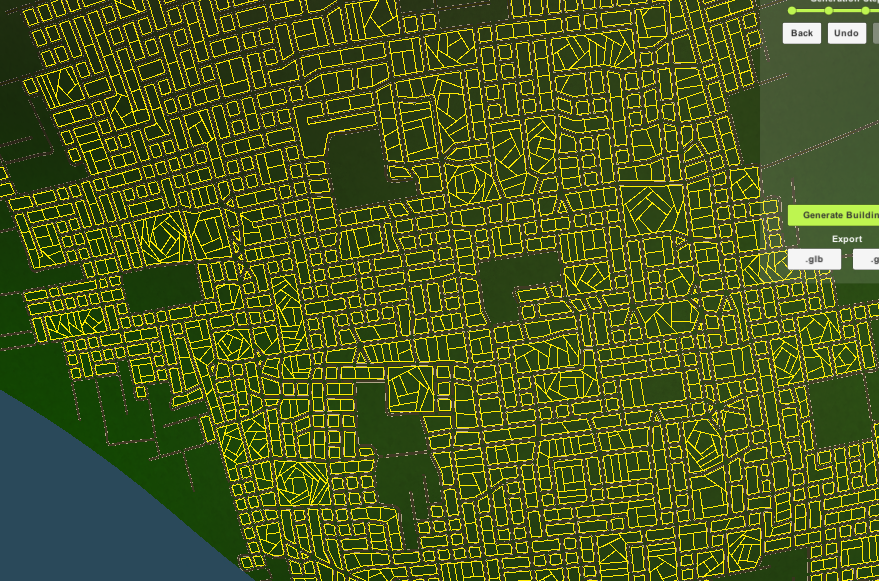
\includegraphics[width=0.8\textwidth]{figure/plot.png}
  \caption{Generated plots within a larger city.}

  \label{fig:plot}
\end{figure}

Each plot is assigned a plot label, which is later used for the PlotContentGenerator to determine what should be generated within the plot.
The plot labels are \textit{Manhattan}, \textit{Skyscraper}, \textit{Park}, \textit{Parking}, and \textit{Empty}.
\textit{Manhattan} and \textit{Skyscraper} are two different sub-generators for BuildingGenerator. 
\textit{Park} and \textit{Parking} are used by the ParkGenerator and the ParkingGenerator respectively.
If the plot label is \textit{Empty}, then no content is generated upon the plot. 

\section{Building Generation}


Building generation produces two different types of buildings: one for plots labeled \textit{Manhattan}, and one for those labeled \textit{Skyscraper}. 
An example of a skyline shaped by these buildings is shown in Figure \ref{fig:skyline-result}.

\begin{figure}[H]
  \centering

  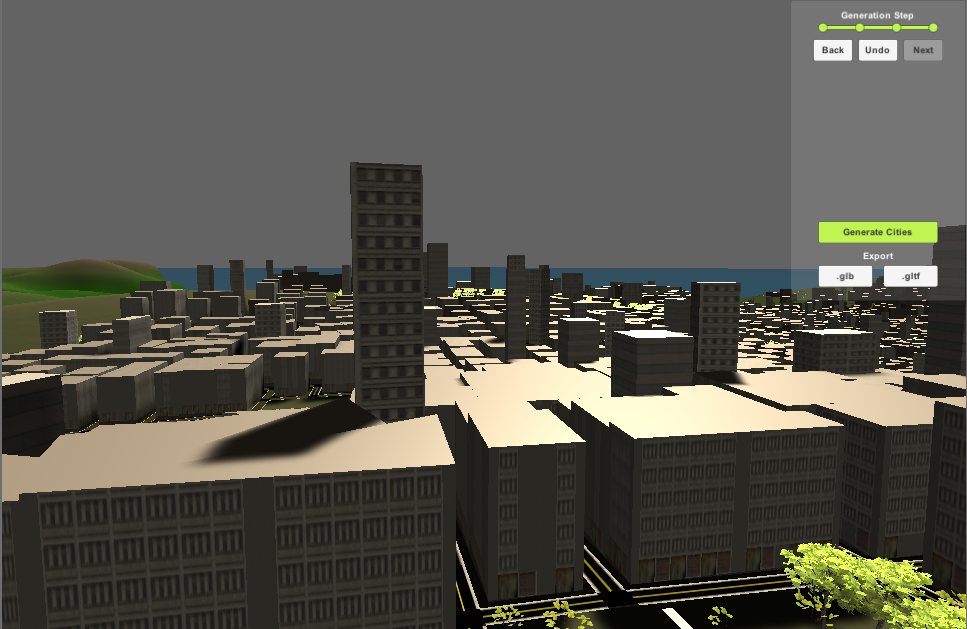
\includegraphics[width=0.7\textwidth]{figure/skyline.PNG}
  \caption{Skyline of \textit{Manhattan} and \textit{Skyscraper} buildings together, taller buildings being the skyscrapers}

  \label{fig:skyline-result}
\end{figure}

\textit{Manhattan} buildings are generated with stochastic L-systems, providing versatility via modular floor-type and wall-type L-systems.
The final implementation had one floor-type and four wall-type generators, Figure \ref{fig:wall-segment-generator} shows examples of this in action.
\textit{FirstFloor} is the first floor type for every building, its wall segment generator produces a combination of shop windows, walls, and doors.
After the \textit{FirstFloor}, the floor-type generator repeats one of the following floor-type until the desired building height has been reached.
Note that each floor-type has its own wall segment generator that is run once per wall, and copied for each floor. 

\begin{itemize}
  \item \textit{NormalFloor} - generates wall and window segments, but it only generates half of the wall. For the other half, it copies the first half and reverses it. 
  \item \textit{EveryOtherFloor} - alternates between wall and window segments.
  \item \textit{RepeatWindowFloor} - only generates window segments.
\end{itemize}

Each of these strategies also start and end with a corner segment. 

\begin{figure}[H]
  \centering

  \begin{subfigure}[b]{0.3\textwidth}
    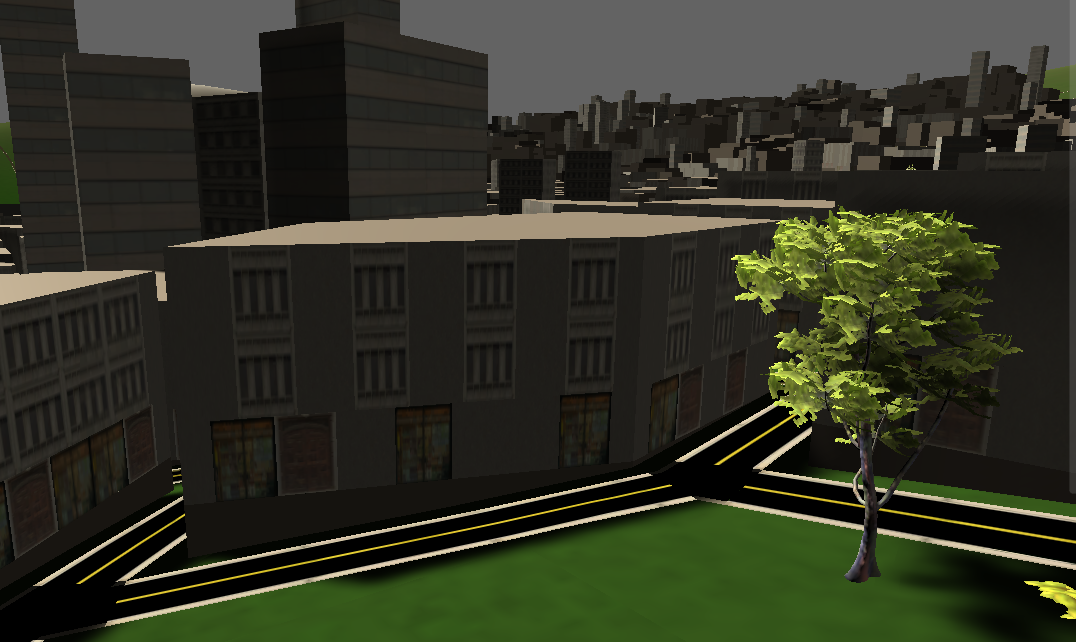
\includegraphics[width=\textwidth]{figure/building-every-other.PNG}
    \caption{\textit{EveryOtherFloor}.}
  \end{subfigure}
  \quad
  \begin{subfigure}[b]{0.3\textwidth}
    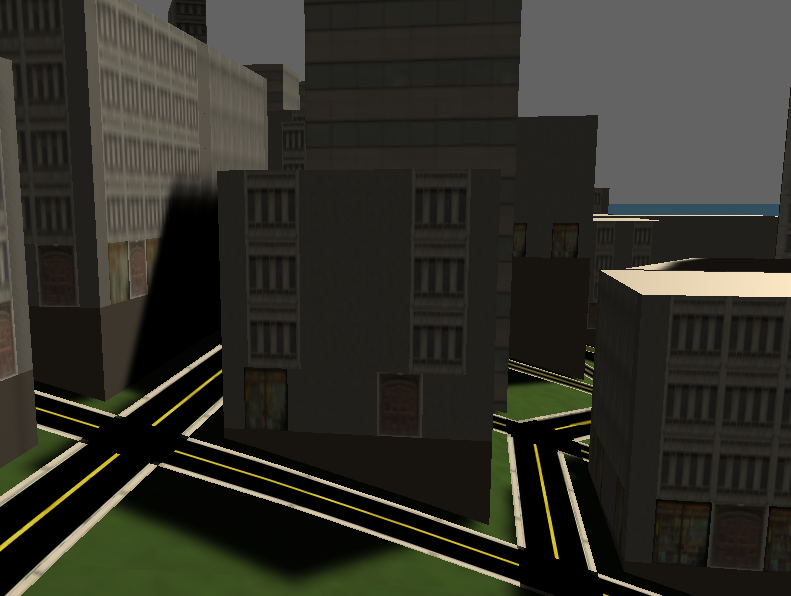
\includegraphics[width=\textwidth]{figure/building-normal.PNG}
    \caption{\textit{NormalFloor}.}
  \end{subfigure}
  \quad
  \begin{subfigure}[b]{0.3\textwidth}
      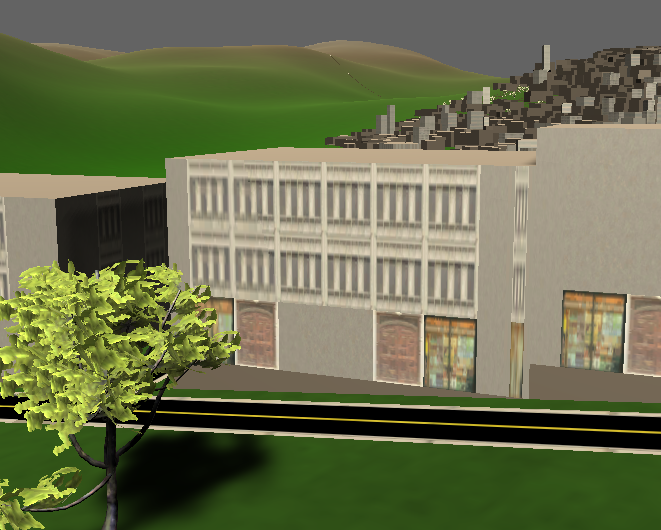
\includegraphics[width=\textwidth]{figure/building-only-window.PNG}
      \caption{\textit{RepeatWindowFloor}.}
  \end{subfigure}
  
  \caption{The three different wall segment generators. Notice that each building has a \textit{FirstFloor} wall segment generator on the first floor.}
  \label{fig:wall-segment-generator}
\end{figure}

The other building type is \textit{Skyscraper}, of which examples are shown in Figure \ref{fig:skyscraper-result}.
These buildings use texture atlases of windows from which different sub-regions are sampled to produce a procedural pattern of random windows.

\begin{figure}[H]
  \centering

  \begin{subfigure}[b]{0.45\textwidth}
    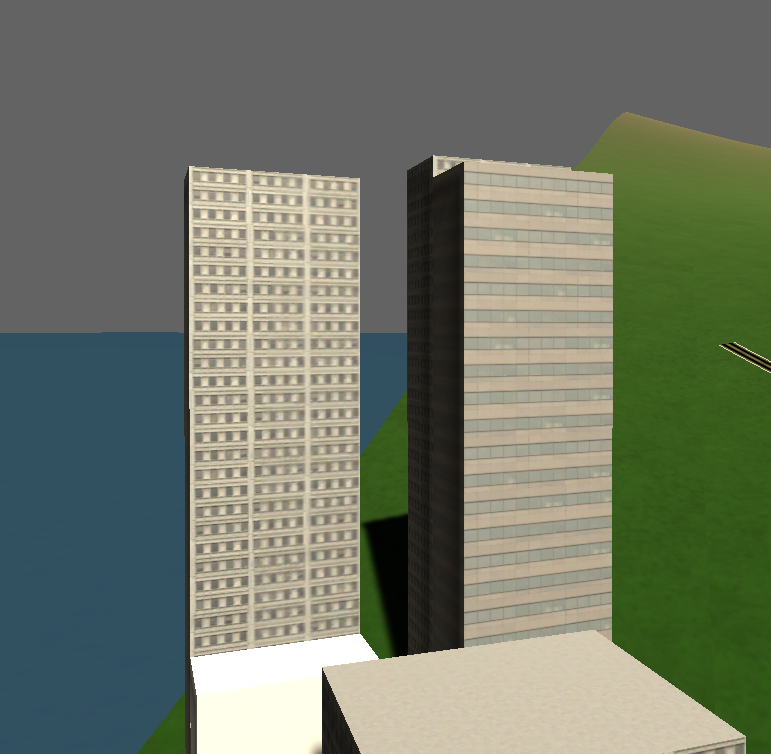
\includegraphics[width=\textwidth]{figure/skyscraper-close-up.PNG}
  \end{subfigure}
  \quad
  \begin{subfigure}[b]{0.45\textwidth}
    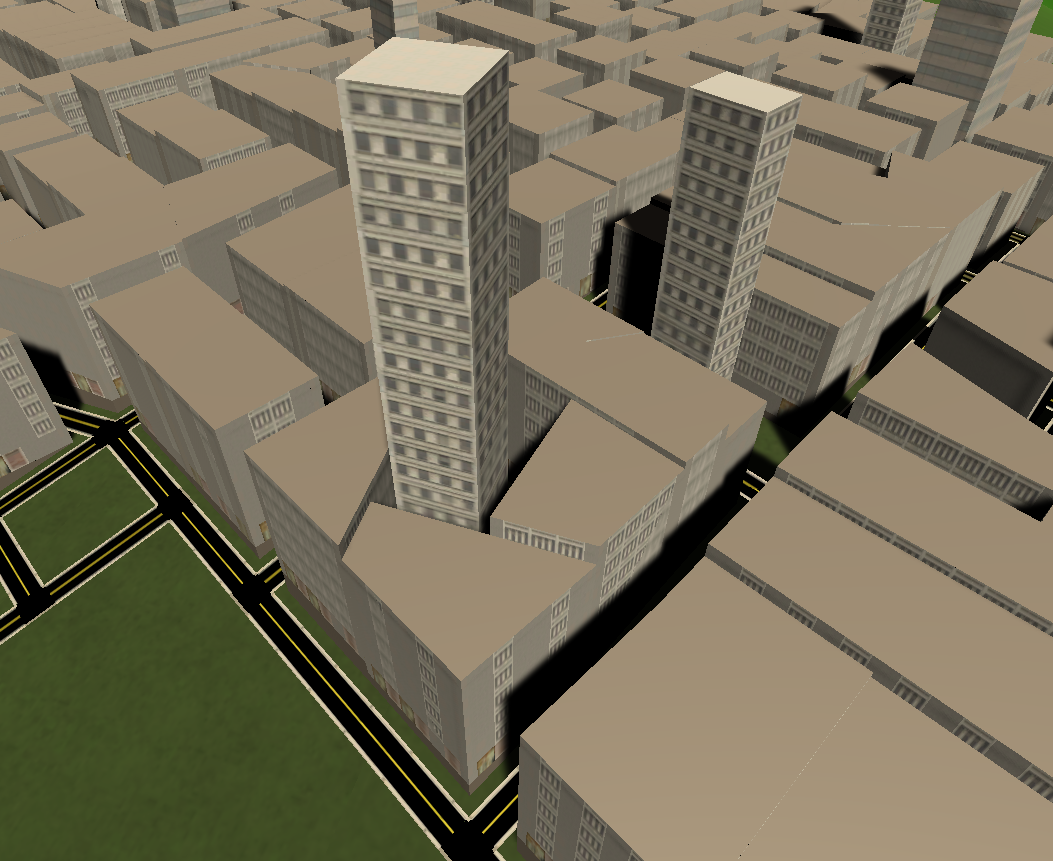
\includegraphics[width=\textwidth]{figure/wack.PNG}
  \end{subfigure}

  \caption{Two examples of skyscrapers generated in a city.}
  \label{fig:skyscraper-result}
\end{figure}

\section{Park Generation}

Once the plot generation is finished the park generation starts working to fill the generated plots with parks.

The parks are generated through two steps, the first step is to generate a natural looking path, and the second step is to fill the park with objects such as trees, bushes, and rocks. 
The algorithm for paths works by firstly generating a random point on one of the edges of the plot and then scattering points randomly, although with a minimum distance from one another, across the plot. 
Secondly the points are sorted by distance, ensuring that the path always traverses to the closest possible point. 
Finally once all points are found the algorithm either creates a path that loops back to the starting point, or a path towards another random point on the edge of the plot (see ~Figure\ref{fig:parks}).

The algorithm for object placement runs after the one for creating paths as the objects have to take the coordinates of the path into consideration.
The first step of the object placement algorithm is to assign each object-type with an object radius, indicating the distance at which other objects are allowed to be created. 
Afterward, a probability of being generated is assigned to each object-type.
The algorithm then runs a number of times and each time an object-type is picked, a model of that object-type is randomly chosen, scaled, and rotated before being generated and placed somewhere in the park.

\begin{figure}[H]
  \centering
  \begin{subfigure}[b]{0.4\textwidth}
    \frame{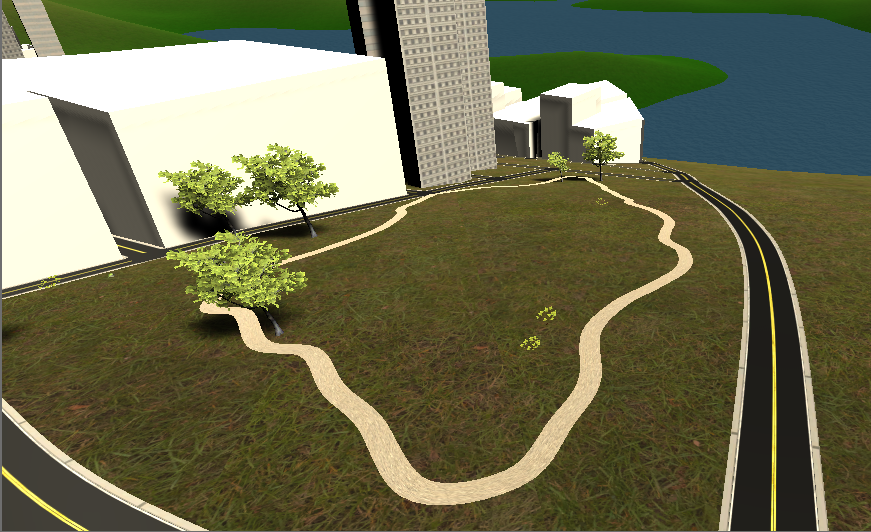
\includegraphics[width=\textwidth]{figure/loopy}}
    \caption{Park with looping path.}
  \end{subfigure}
  \quad
  \begin{subfigure}[b]{0.4\textwidth}
    \frame{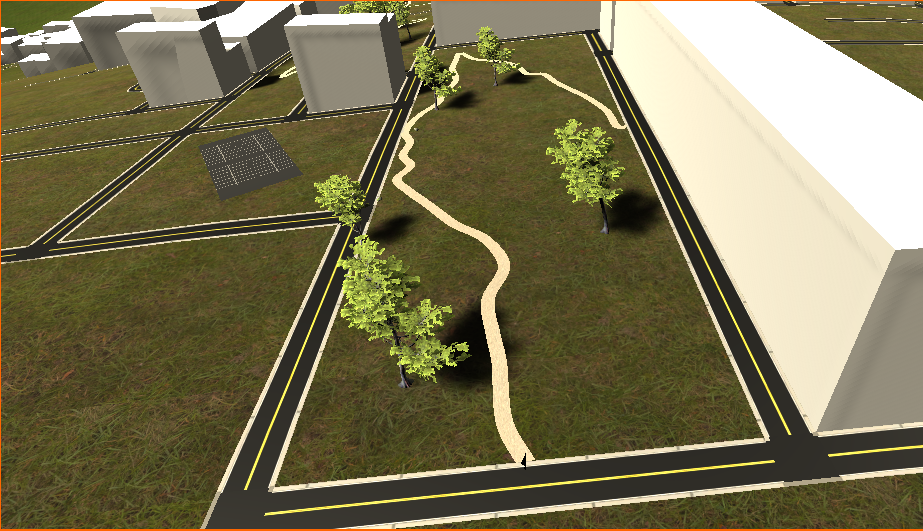
\includegraphics[width=\textwidth]{figure/path}}
    \caption{Park with path that does not loop.}
  \end{subfigure}
  \caption{Two example of different generated parks. One with a path that loops back, and one that creates a path to another edge of the plot.}
  \label{fig:parks}
\end{figure}
 
It is worth noting that even though the paths always end up looping, or connecting to a random edge, their shapes still vary a lot, leading to quite interesting results (see Figure~\ref{fig:park_ex2}).
The fact that object placement takes the path into consideration also make the park layout appear less random and more relative to its environment. 
This provides a more consistent feeling to the different parks.
 
\begin{figure}[H]
  \centering
  \begin{subfigure}[b]{0.4\textwidth}
    \frame{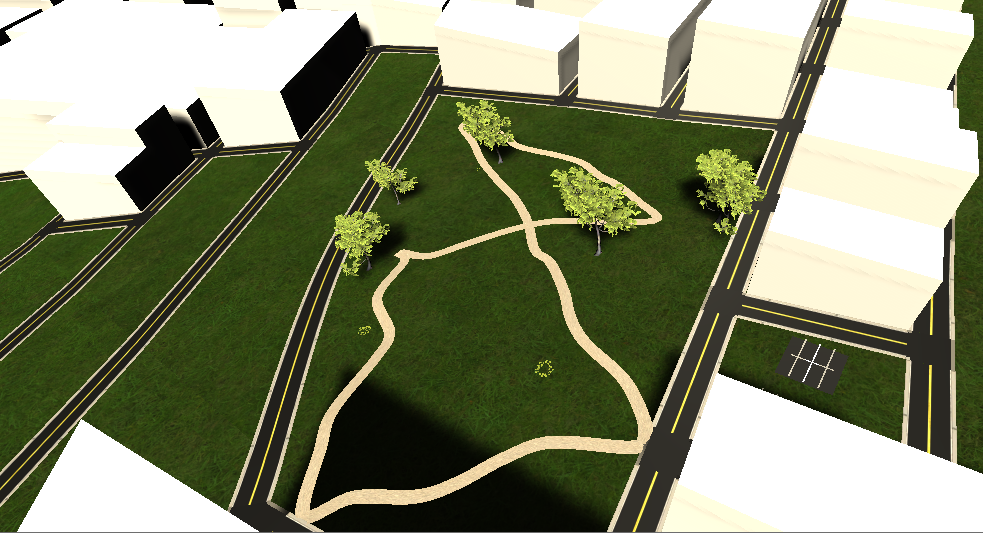
\includegraphics[width=\textwidth]{figure/loopytwo}}
  \end{subfigure}
  \quad
  \begin{subfigure}[b]{0.4\textwidth}
    \frame{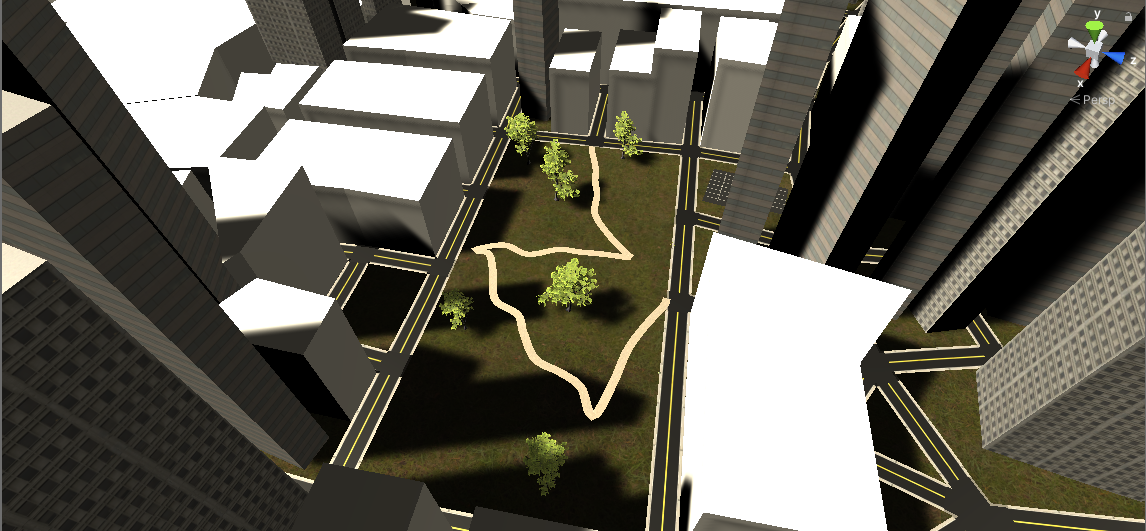
\includegraphics[width=\textwidth]{figure/nonlooptwo}}
  \end{subfigure}
  \caption{Two additional examples, showcasing different results.}
  \label{fig:park_ex2}
\end{figure}
 
\section{Parking Lot Generation}

Once the plot generation is finished the parking lot generation starts to fill some of the generated plots with parking lots.
The generated parking lots consist of one or more rows of parking spaces (see Figure~\ref{fig:results_parking_sizebased}).

\begin{figure}[H]
   \centering
   \begin{subfigure}[b]{0.38\textwidth}
     \frame{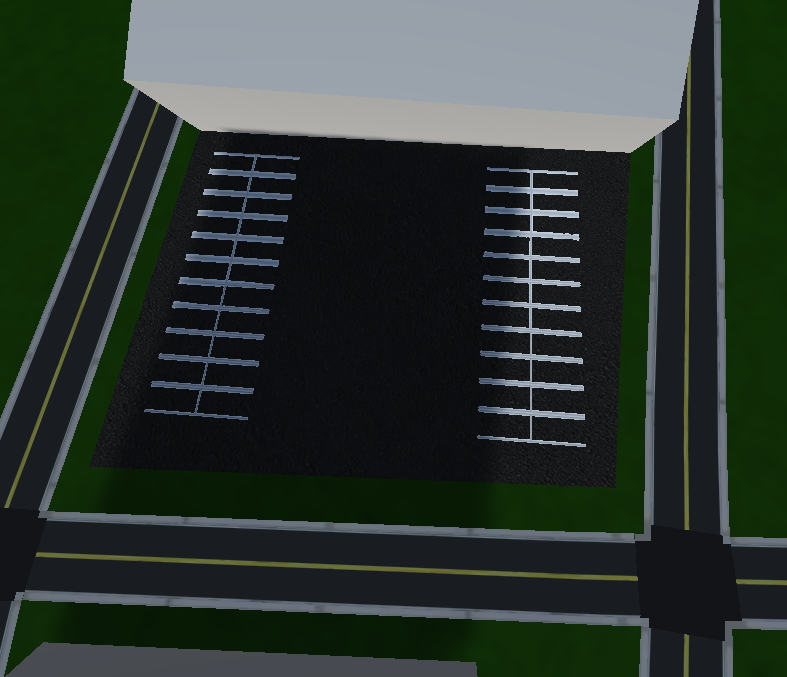
\includegraphics[width=\textwidth]{figure/results/parking/bigplot}}
     \caption{Large parking lot consisting of two rows.}
   \end{subfigure}
   \quad
   \begin{subfigure}[b]{0.52\textwidth}
     \frame{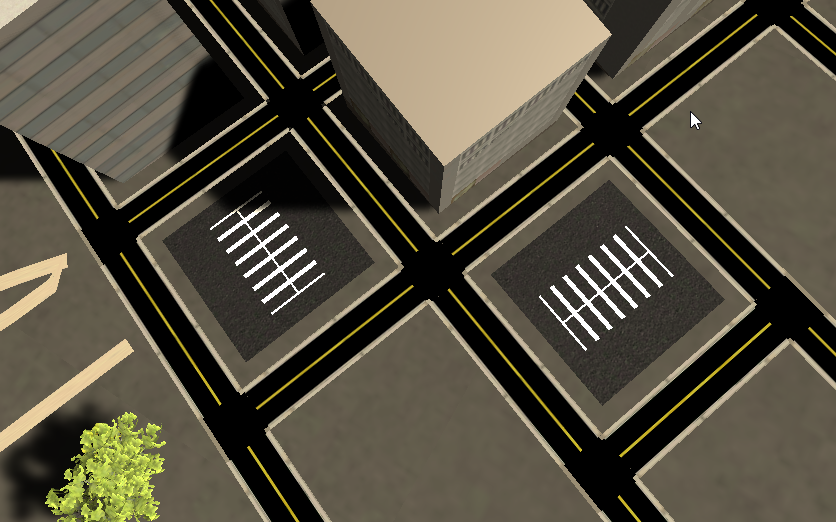
\includegraphics[width=\textwidth]{figure/results/parking/smallplots}}
     \caption{Two small parking lots consisting of one row.}
   \end{subfigure}
     \caption{Two examples of different sized parking lots created by the generator.}
   \label{fig:results_parking_sizebased}
 \end{figure}

These parking lots are generated by approximating the largest possible rectangle that fits inside a given plot, and then generating parking lots inside of it.
The number of rows is based on the size of the computed rectangle, and the algorithm aims to fit as many rows of parking lots inside the rectangle such that there still exists space between the rows for cars to enter.

Having the parking lots consist of multiple rows depending on the size gives some more variety, but the decision to do this was also based on real-world parking lots (see Figure~\ref{fig:parkings}).
In the left example in Figure~\ref{fig:parkings}, a road is used to separate parking spaces, making it impossible for parked cars to be surrounded and stuck by other parked cars.
The right example, however, has a more interesting shape, the parking lot in the center of it is shaped in the two-row style, while the surrounding rectangle is large enough that cars can easily drive around and not be blocked by parked cars.
This type of parking space is difficult to generate reliably in arbitrary plot shapes, consequently shapes like these were left out of the scope for this project.
